\chapter{Network Bending: Direct and Expressive Manipulation of Generative Neural Networks}
\label{ch:net_bend}

\section{Introduction}

This chapter details the development of the \textit{network bending} framework. Which is a way to directly manipulate the internal features of generative neural networks during inference (Fig. \ref{fig:c5:overview_diagram} for an overview). This work was first published online as a pre-print on arxiv \citep{broad2020network}, then later a revised manuscript was accepted as a conference paper at EvoMUSART \citep{broad2021network}, and then as an extended journal paper in Entropy \citep{broad2022network}.
The experiments in the original paper were applied to the task of image generation with StyleGAN2 on models that were pre-trained on the FFHQ (Flickr-Faces High-Quality) \citep{karras2019analyzing} and LSUN (Large-scale Scene UNderstanding) churches dataset \citep{yu2015lsun}. 
A follow-up study applying the same techniques to audio using a custom VAE trained on a dataset of varied musical genres (\S \ref{c5:sec:net-bend-audio}) was later completed for the extended Entropy paper. 
In this chapter, these experiments are documented chronologically.


\begin{figure}[!htb]
    \centering
    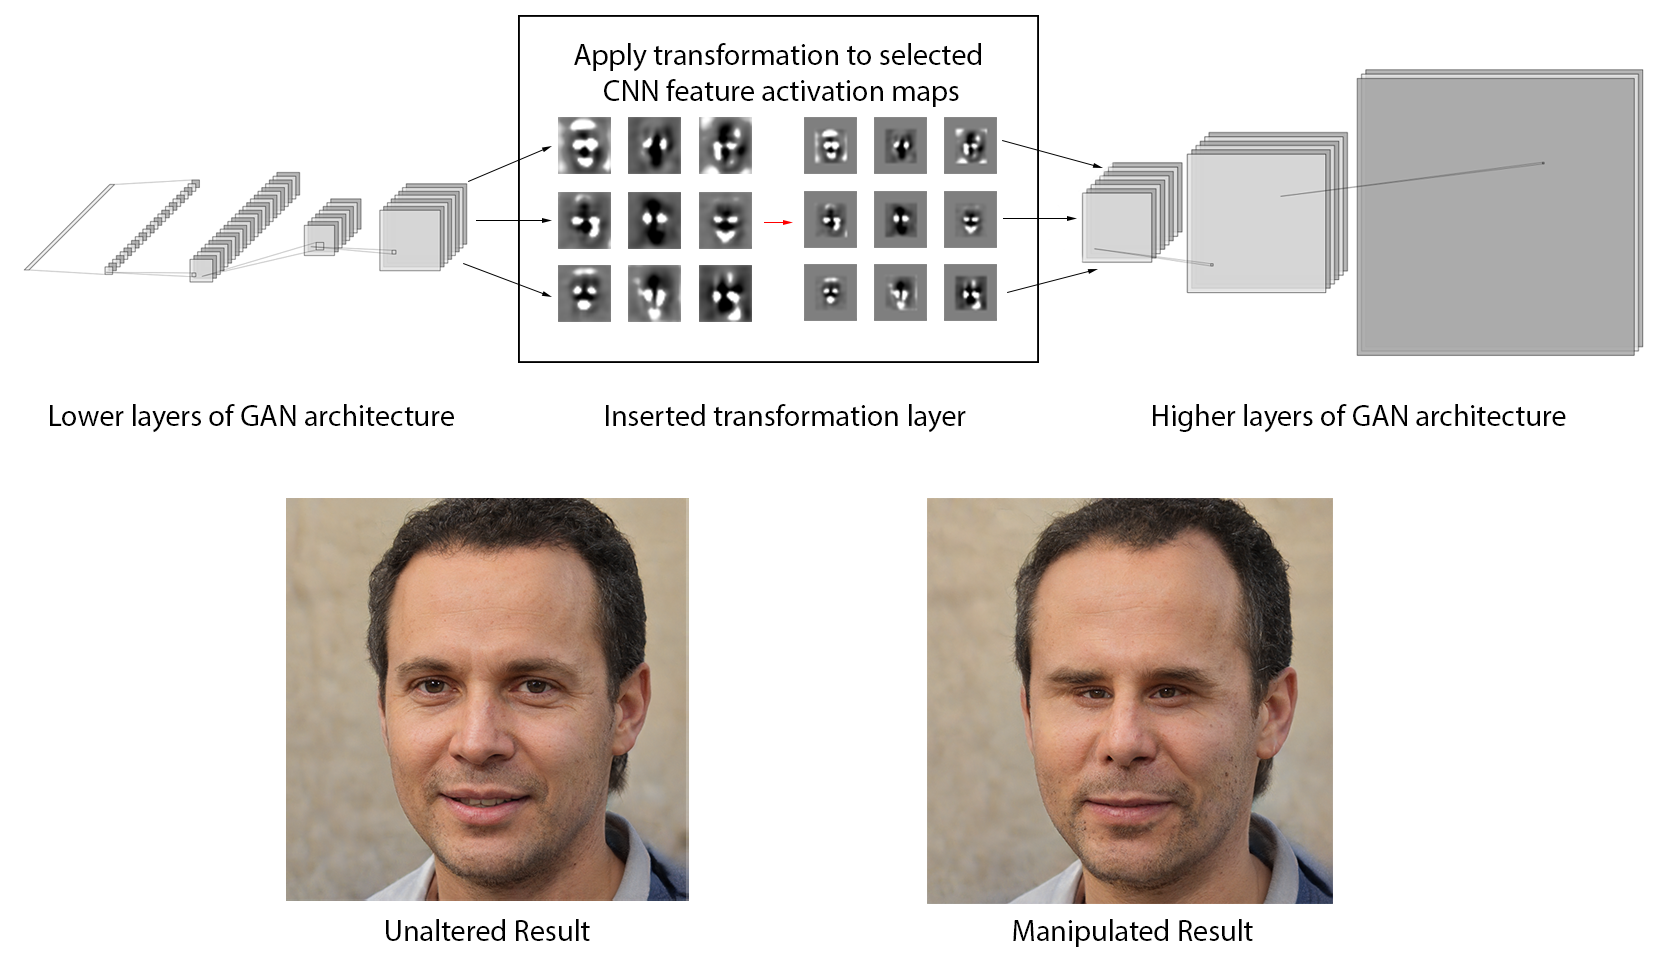
\includegraphics[width=1\textwidth]{figures/c5_netbend/misc/network-bending-diagram.png}
    \caption[Visual overview of the \textit{network bending} framework]{Visual overview of the \textit{network bending} framework, where deterministically controlled transformation layers can be inserted into a pre-trained network. As an example, a transformation layer that scales the activation maps by a factor of $k_x=k_y=0.6$ is applied (\S\ref{sec:affine}) to a set of features in layer 5 responsible for the generation of eyes, which has been discovered in an unsupervised fashion using the clustering algorithm to cluster features based on the spatial similarity of their activation maps (\S \ref{c5:sec:clustering}). Bottom left shows the sample generated by StyleGAN2 \citep{karras2019analyzing} trained on the FFHQ dataset without modification, while the image on the right shows the same sample generated with the scaling transform applied to the selected features. NB: the GAN network architecture diagram shown on the top row is for illustrative purposes only.}
    \label{fig:c5:overview_diagram}
\end{figure}

\section{Motivation}

Following the experiments detailed in Chapters \ref{ch:unstable_eq} \& \ref{ch:divergent}, I wanted to find an approach for actively diverging from data with generative neural networks, that was easier to control than methods that required directly training or fine-tuning the network itself.
In addition, whilst producing novel outputs, the previous approaches did not necessarily expand the possibility space of what could be generated in a way that was arguably superior to traditional generative modelling.
Both previous approaches focus on learning a set of weights that lead to reduced diversity in the generated outputs when compared with the successful training of a standard generative model such as a GAN or VAE.
The goal of the work described in this chapter was to find an approach that would expand the generative space, not shrink it. 


The inspiration for \textit{network bending} came from a conversation with my supervisor Mick Grierson.
After showing him the results detailed in the previous chapters, he said that though he liked the results, he was interested in methods that were more interactive and controllable, saying something along the lines of `I just want to stick my hand in the model and squeeze it, and see what pops out the other side' \citep{grierson2020personal}\footnote{According to Mick Grierson, the idea for network bending was also being discussed in MIMIC (Musically Intelligent Machines Interacting Creatively) research team meetings around the same time. As I was not involved in those meetings, I cannot give a clear chronology of events.}. 
This statement stuck with me and eventually led to the development of the framework described here.

In some of the early experiments that led to this work, I hard-coded simple transformations into StyleGAN1 \citep{karras2019style} models during inference.
These early experiments (which later went on to become the series of artworks \textit{Teratome} \S \ref{c7:subsubsec:teratome}) sparked the intuition that eventually led to the implementation of many kinds of transformation layers (\S \ref{c5:sec:transforms}) and the clustering approach for grouping features together (\S \ref{c5:sec:clustering}).
The motivation for developing the clustering algorithm was the observation that when transformations were applied to random subsets of convolutional filters in a layer, then in some instances, manipulation of groups of filters had apparently powerful semantic effects, that could not be captured my only manipulating individual filters, as was done in the approach presented by \citep{bau2019semantic}.

In creating this framework, I wanted to give as much control and agency to people to manipulate generative neural networks as possible. 
The flexibility of this framework was key in order to achieve this, allowing for the expansion of the generative space of generative neural networks in a data-divergent fashion

\section{Transformation Layers}

\label{c5:sec:transforms}

A key goal in this framework was to give as much direct control and agency to artists and creatives as possible.
To maximise the amount of control people could have, I implemented a broad variety of deterministically controlled transformation layers that can be dynamically inserted into the computational graph of the generative model. 
The transformation layers are implemented natively in PyTorch \citep{paszke2019pytorch} for speed and efficiency. I
 treated the activation maps of each feature of the generative model as 1-channel images in the range -1 to 1. 
 Each transformation is applied to the activation maps individually before they are passed to the next layer of the network. 

 The transformation layers can be applied to all the features in a layer, or a random selection, or by using pre-defined groups automatically determined based on spatial similarity of the activation maps (\S \ref{c5:sec:clustering}). 
 Figure \ref{fig:c5:layerwide_comparison} shows a comparison of a selection of these transformations applied to all the features layer-wide in various layers of StyleGAN2.

\begin{figure}[htbp]
    \centering
    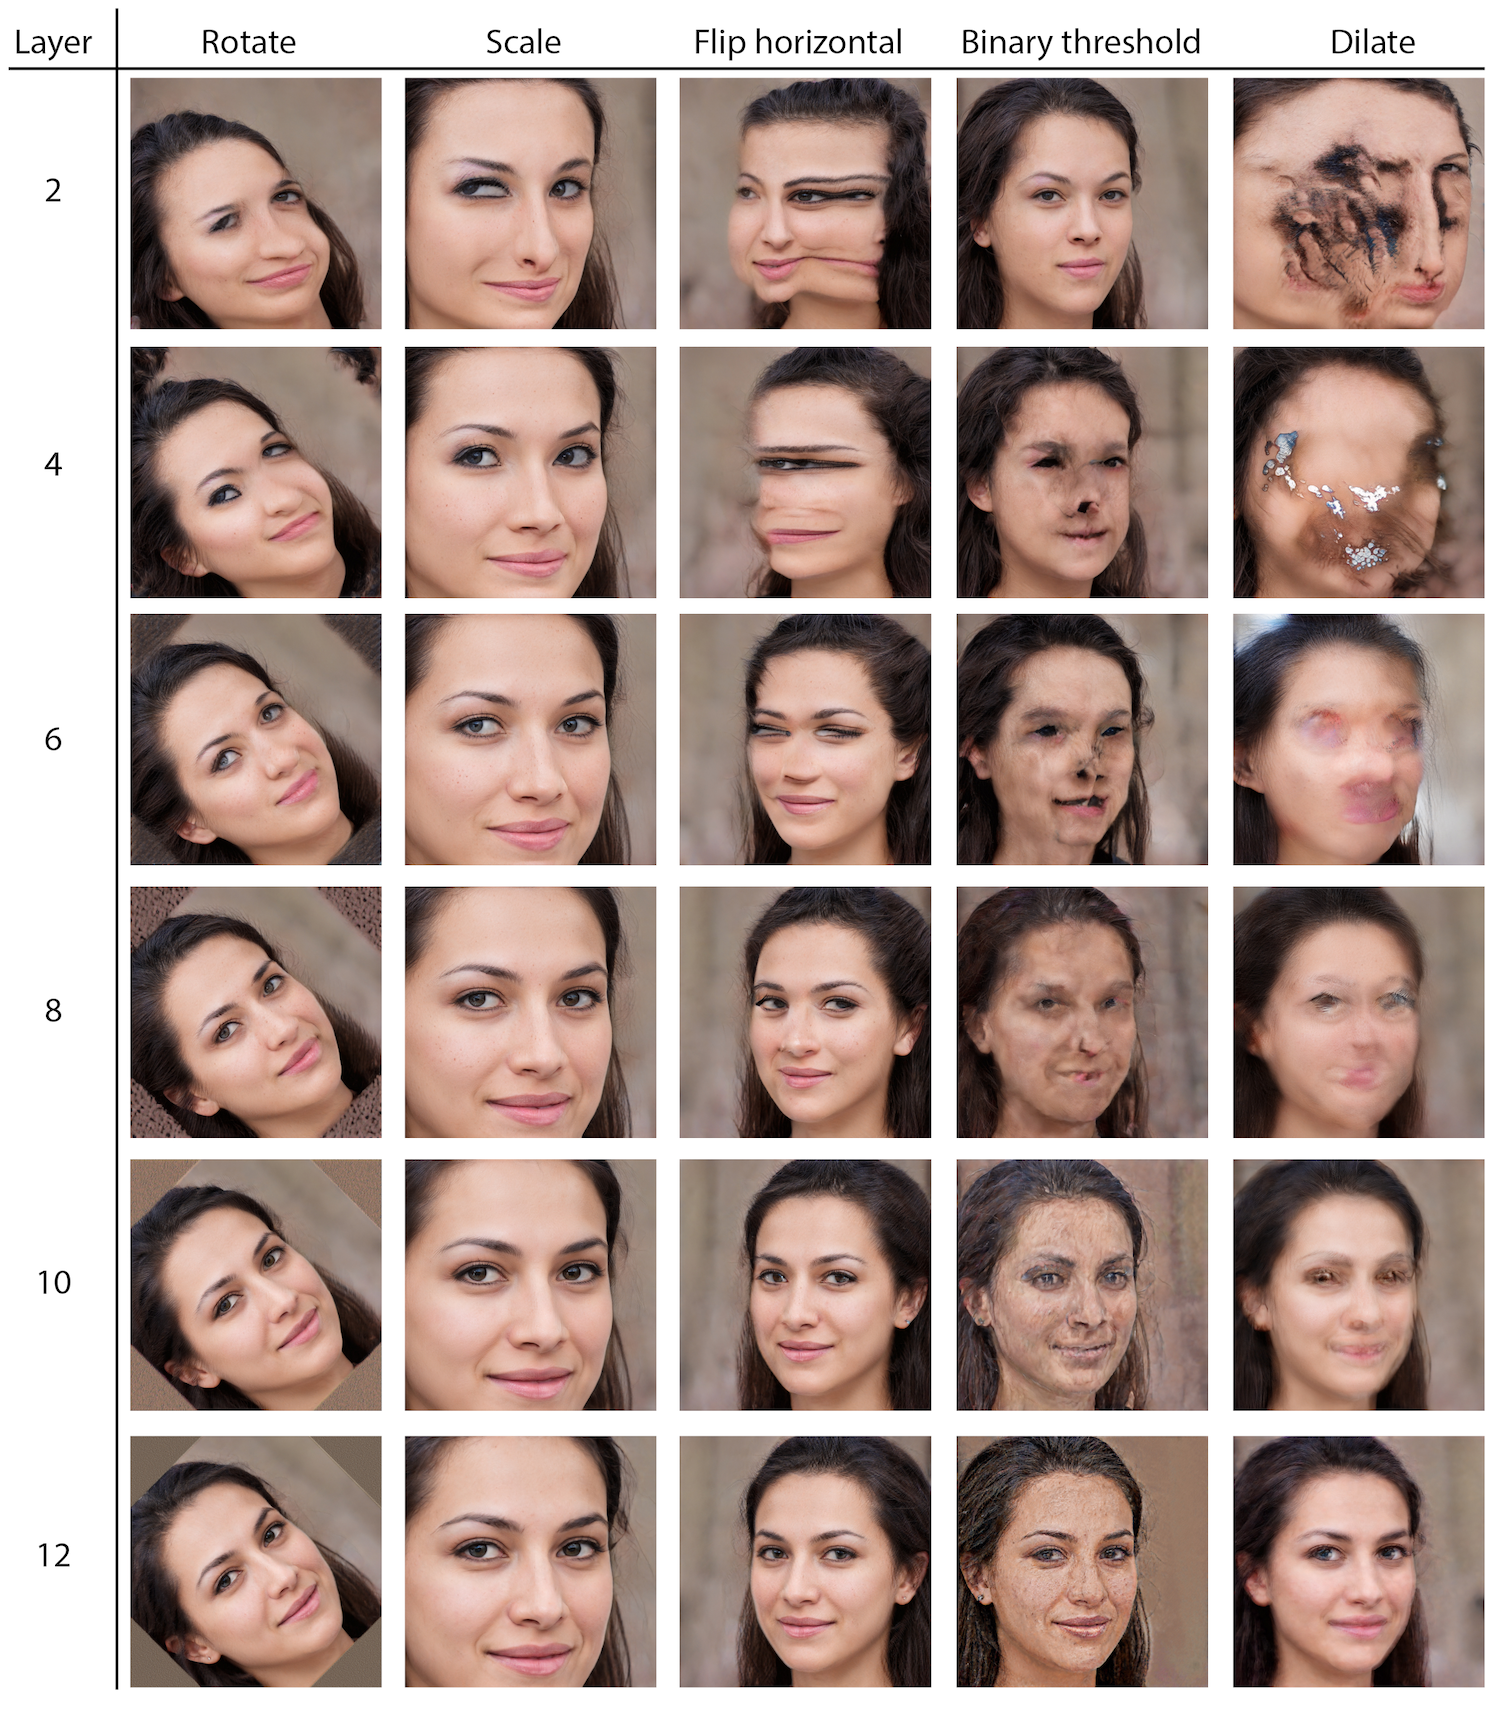
\includegraphics[width=1\textwidth]{figures/c5_netbend/misc/transform-comparison.png}
    \caption[Comparsion of various transformation layers applied in different layers of StyleGAN2]{A comparison of various transformation layers inserted and applied to all of the features in different layers in the StyleGAN2 network trained on the FFHQ dataset, showing how applying the same filters in different layers can make wide-ranging changes the generated output. The rotation transformation is applied by an angle $\theta=45$. The scale transformation is applied by a factor of $k_{x}=k_{y}=0.6$. The binary threshold transformation is applied with a threshold of $t=0.5$. The dilation transformation is applied with a structuring element with radius $r=2$ pixels.}
    \label{fig:c5:layerwide_comparison}
\end{figure}


\subsection{Pointwise Transformations}

I began with simple pointwise numerical transformations $f(x)$ that are applied to individual activation units $x$. 
I implemented four distinct numerical transformations: the first is \emph{ablation}, which can be interpreted as $f(x) = x \cdot 0$. 
The second is \emph{inversion}, which is implemented as $f(x) = 1 - x$. 
The third is \emph{multiplication by a scalar} $p$ implemented as $f(x) = x \cdot p$. 
The final transformation is \emph{binary thresholding} (often referred to  as posterisation) with threshold $t$, such that:
\begin{equation}
f(x) = \begin{cases}
    1,& \text{if  } x\geq t\\
    0,              & \text{otherwise}
\end{cases}
\end{equation}

\subsection{Affine Transformations}
\label{sec:affine}
For this set of transformations, each activation map $X$ for feature $f$ is treated as an individual matrix that simple affine transformations can be applied to. 
The first two are horizontal and vertical \emph{reflections} that are defined as:
\begin{equation}
X \begin{bmatrix}
-1 & 0 & 0\\
\ 0 & 1 & 0\\
\ 0 & 0 & 1
\end{bmatrix}\quad , \quad X \begin{bmatrix}
1 & \ 0 & 0\\
0 & -1 & 0\\
0 & \ 0 & 1
\end{bmatrix}
\end{equation}

\noindent The second is \emph{translations} by parameters $p_x$ and $p_y$ such that:
\begin{equation}
X \begin{bmatrix}
1 & 0 & p_x\\
0 & 1 & p_y\\
0 & 0 & 1
\end{bmatrix}
\end{equation}

\noindent The third is \emph{scaling} by parameters $k_x$ and $k_y$ such that:
\begin{equation}
X \begin{bmatrix}
k_x & 0 & 0\\
0 & k_y & 0\\
0 & 0 & 1
\end{bmatrix}
\end{equation}
Note that in this chapter, I only report on using uniform scalings, such that $k_x = k_y$. Finally, fourth is \emph{rotation} by an angle $\theta$ such that:
\begin{equation}
X \begin{bmatrix}
cos(\theta) & -sin(\theta) & 0\\
sin(\theta) & cos(\theta) & 0\\
0 & 0 & 1
\end{bmatrix}
\end{equation}

\subsection{Morphological Transformations}

I implemented two of the possible basic mathematical morphological transformation layers, performing \emph{erosion} and \emph{dilation} \citep{soille1999erosion} when applied to the activation maps, which can be interpreted as 1-channel images  (Fig. \ref{fig:c5:morphological transforms}). 
These can be configured with the parameter $r$ which is the radius for a circular kernel (aka structural element) used in the morphological transformations.

\begin{figure}[!htb]
    \centering
    \subfloat[]{\label{subfig:morph-a}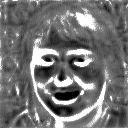
\includegraphics[width=.32\textwidth]{figures/c5_netbend/morphology_activations/original_007.png}}
    \hfill
    \subfloat[]{\label{subfig:morph-a-erode}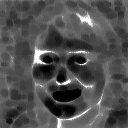
\includegraphics[width=.32\textwidth]{figures/c5_netbend/morphology_activations/erode_007.png}}
    \hfill
    \subfloat[]{\label{subfig:morph-a-dilate}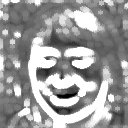
\includegraphics[width=.32\textwidth]{figures/c5_netbend/morphology_activations/dilate_007.png}}
    \caption[Examples of morphological transformations being applied to an individual activation map in Layer 10 of StyleGAN2]{Examples of morphological transformations being applied to an individual activation map in Layer 10 of StyleGAN2. (a) Unmodified activation maps. (b) Activation map after erosion was applied ($r=2$ pixels). (c) Activation maps after dilation were applied ($r=2$ pixels).}
    \label{fig:c5:morphological transforms}
 \end{figure}

\section{Clustering Features}
\label{c5:section:clustering}

As most of the layers in the current state-of-the-art generative models, such as StyleGAN2, have very large numbers of convolutional features, controlling each one individually would be far too complicated to build a user interface around and control these in a meaningful way. 
In addition, because of the redundancy existing in these models, manipulating individual features does not normally produce any kind of meaningful outcome.\footnote{I discovered this through my early hard-coded experiments with network bending that are discussed in Section \ref{c7:subsubsec:teratome}.} 
Therefore, it is necessary to find some way of grouping them into more manageable ensembles of sets of features. 
Ideally, such sets of features would correspond to the generation of distinct, semantically meaningful aspects of the image, and manipulating each set would correspond to the manipulation of specific semantic properties in the resulting generated sample. 
To achieve this, I developed a novel approach that combines metric learning and a clustering algorithm to group sets of features in each layer based on the spatial similarity of their activation maps. 
I trained a separate convolutional neural network (CNN) for each layer of StyleGAN2 to analyse the appearance of the activation maps. 
The CNN has a bottleneck architecture (first introduced by Gr{\'e}zl et al.~\citep{grezl2007probabilistic}) to learn a highly compressed feature representation; the latter is then used in a metric learning approach in combination with the $k$-means clustering algorithm \citep{lloyd1982least, celebi2013comparative} to group sets of features in an unsupervised fashion. 

\subsection{Architecture}

For each layer of StyleGAN2, I trained a separate CNN on the activation maps of all the convolutional features. 
The resolution of the activation maps and the number of convolutional features varies for the different layers of the model (a breakdown of which can be seen in Table \ref{tab:classifier-table}).
I employed an architecture that can dynamically be changed, by increasing the number of convolutional blocks, depending on what depth is required. 

\begin{table}[]
\centering
\begin{tabular}{|c|c|c|c|c|c|}%{llllll}
\hline
Layer & Resolution & \#features &  CNN depth & \#clusters & Batch size\\
\hline
1     & 8x8        & 512          & 1                & 5                & 500        \\
2     & 8x8        & 512          & 1                & 5                & 500        \\
3     & 16x16      & 512          & 2                & 5                & 500        \\
4     & 16x16      & 512          & 2                & 5                & 500        \\
5     & 32x32      & 512          & 3                & 5                & 500        \\
6     & 32x32      & 512          & 3                & 5                & 500        \\
7     & 64x64      & 512          & 4                & 5                & 200        \\
8     & 64x64      & 512          & 4                & 5                & 200         \\
9     & 128x128    & 256          & 5                & 4                & 80         \\
10    & 128x128    & 256          & 5                & 4                & 80         \\
11    & 256x256    & 128          & 6                & 4                & 50         \\
12    & 256x256    & 128          & 6                & 4                & 50         \\
13    & 512x512    & 64           & 7                & 3                & 20         \\
14    & 512x512    & 64           & 7                & 3                & 20         \\
15    & 1024x1024  & 32           & 8                & 3                & 10         \\
16    & 1024x1024  & 32           & 8                & 3                & 10       \\
\hline
\end{tabular}
\medskip
\caption[Table detailing model architecture for the ShuffleNet models used for clustering in StyleGAN2.]{
    \label{tab:classifier-table}Table showing resolution, number of features of each layer, the number of ShuffleNet \citep{zhang2018shufflenet} convolutional blocks for each CNN model used for metric learning, the number of clusters calculated for each layer using $k$-means and the batch size used for training the CNN classifiers for the StyleGAN2 models. Note: LSUN church and cat models have only 12 layers.
%\citep{lloyd1982least, celebi2013comparative}.
}
\end{table}

I employed the ShuffleNet architecture \citep{zhang2018shufflenet} for the convolutional blocks in the network. 
For each convolutional block, I utilised a feature depth of 50 and had one residual block per layer. 
The motivating factor in many of the decisions made for the architecture design was not focused on achieving the best accuracy per se. 
Instead, I wanted a network that could learn a sufficiently good metric while also being reasonably quick to train (with 12-16 separate classifiers required to be trained per the StyleGAN2 model). 
I also wanted a lightweight enough network, such that it could be used in a real-time setting where clusters can quickly be calculated for an individual latent encoding, or when processing large batches of samples.

After the convolutional blocks, I flattened the final layer and used this to learn a mapping into a narrow bottleneck $\vec{v} \in \mathbb{R}^{10}$, before re-expanding the dimensionality of the final layer to the number of convolutional features present in the layer of the respective generative model. 
The goal of this bottleneck is to force the network to learn a highly compressed representation of the different convolutional features in the generative model. 
While this invariably loses some information, most likely negatively affecting classification performance during training, this is in fact the desired result. 
I wanted to force the CNN to combine features of the activation maps with similar spatial characteristics so that they can easily be grouped by the clustering algorithm. 
Another motivating factor is that the chosen clustering algorithm ($k$-means) does not scale well for feature spaces with high dimensionality.

\subsection{Training}

I generated a training set of the activations of every feature for every layer of 1000 randomly sampled images and a test set of 100 samples for the models trained on all of the datasets used in these experiments. 
I trained each CNN using the softmax feature learning approach \citep{dosovitskiy2014discriminative}, a reliable method for distance metric learning. This method employs the standard softmax training regime \citep{bridle1990probabilistic} for CNN classifiers. 
Each classifier has been initialised with random weights and then trained for 100 epochs using the Adam optimiser \citep{kingma2015adam} with a learning rate of 0.0001 and with $\beta_1 = 0.9$ and $\beta_2 = 0.999$. 
All experiments were carried out on a single NVIDIA GTX 1080ti. The batch size used for training the classifiers for the various layers of StyleGAN2 can be seen in Table \ref{tab:classifier-table}. 
% The classifiers for the VAE were all trained with a batch size of 100.

After training, the softmax layer is discarded and the embedding of the bottleneck layer is used as the discriminative feature vector where the distances between points in feature space permit gauging the degree of similarity of two samples. 
This approach differs from standard softmax feature learning as it uses the feature vector from the bottleneck, rather than the last layer prior to softmax classification, giving a more compressed feature representation than the standard softmax feature learning approach.

\subsection{Clustering Algorithm}

\label{c5:sec:clustering}

Once each of the CNNs for every layer has been trained, they can then be used to extract feature representations of the activation maps of the different convolutional features corresponding to each layer of the generative model.
The approach is to perform clustering based on an average of features' embeddings drawn from many random samples, which can be used to find a general-purpose set of clusters for a trained model.

The activation map $X_{df}$ for each layer $d$ and feature $f$ is fed into the CNN metric learning model for that layer $C_d$ to get the feature vector $\vec{v}_{df}$. 
This process is repeated N times (1000 in these experiments) to find the mean feature vector $\vec{\bar{v}}_{df}$ for each convolutional filter.
The mean feature vectors for each filter in each layer are then aggregated and fed to the $k$-means clustering algorithm --- using Lloyd's method \citep{lloyd1982least} with Forgy initialization \citep{forgy1965cluster, celebi2013comparative}. 

The predetermined number of clusters for each layer in StyleGAN2 can be seen in Table \ref{tab:classifier-table}. 
Examples from the clustering algorithm applied to the FFHQ StyleGAN2 model can be seen in Figure \ref{fig:c5:cluster_layer_comp_image}.

\begin{figure}[!htbp]
    \centering
        \subfloat[]{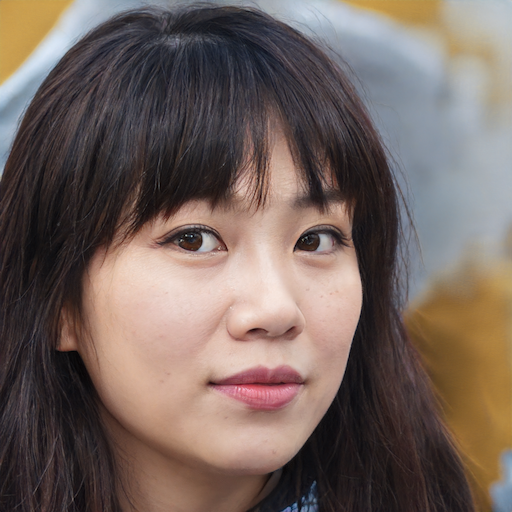
\includegraphics[width=.24\textwidth]{figures/c5_netbend/cluster_comparison/not_manipulated.png}}
        \hfill
        \subfloat[]{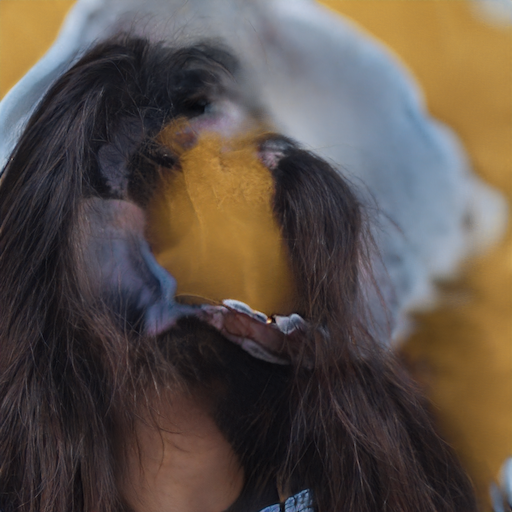
\includegraphics[width=.24\textwidth]{figures/c5_netbend/cluster_comparison/layer_1_cluster0_mult-1.png}}
        \hfill
        \subfloat[]{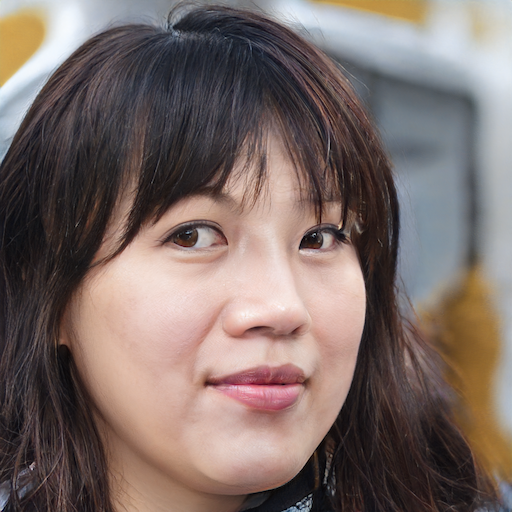
\includegraphics[width=.24\textwidth]{figures/c5_netbend/cluster_comparison/layer_3_cluster2_mult5.png}}
        \hfill
        \subfloat[]{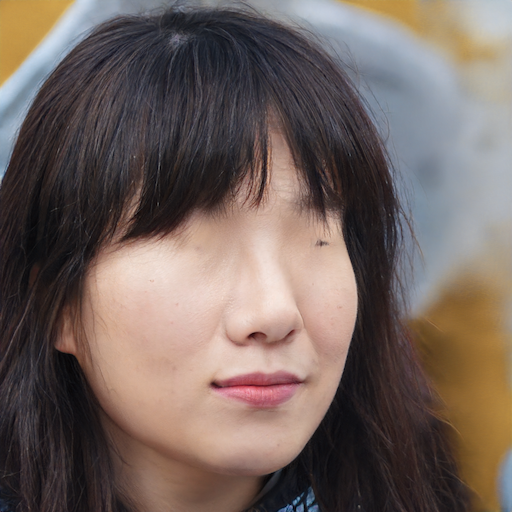
\includegraphics[width=.24\textwidth]{figures/c5_netbend/cluster_comparison/layer_5_cluster2_ablate.png}}
        \hfill
        \subfloat[]{ 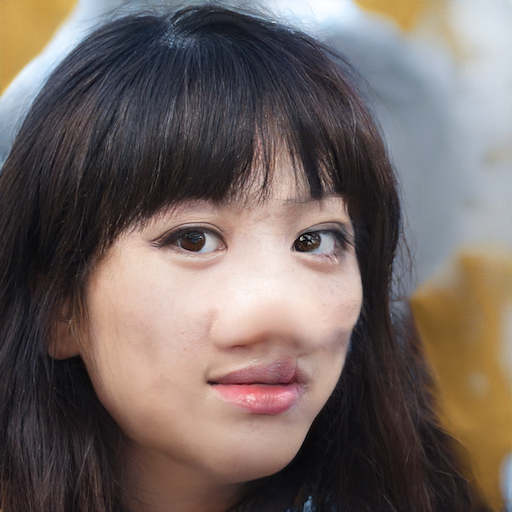
\includegraphics[width=.24\textwidth]{figures/c5_netbend/cluster_comparison/layer_6_cluster4_dilate.png}}
        \hfill
        \subfloat[]{ 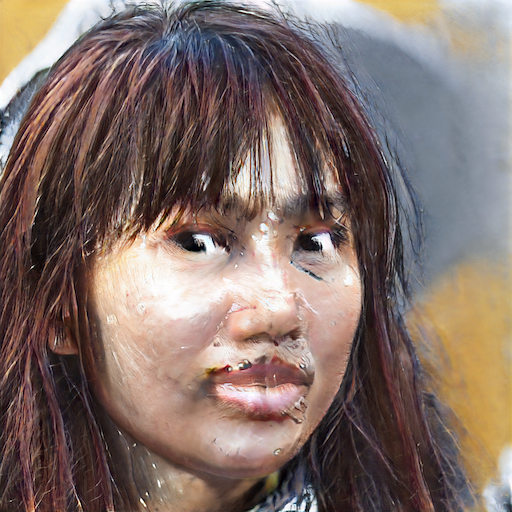
\includegraphics[width=.24\textwidth]{figures/c5_netbend/cluster_comparison/layer_9_cluster3_mult5.png}}
        \hfill
        \subfloat[]{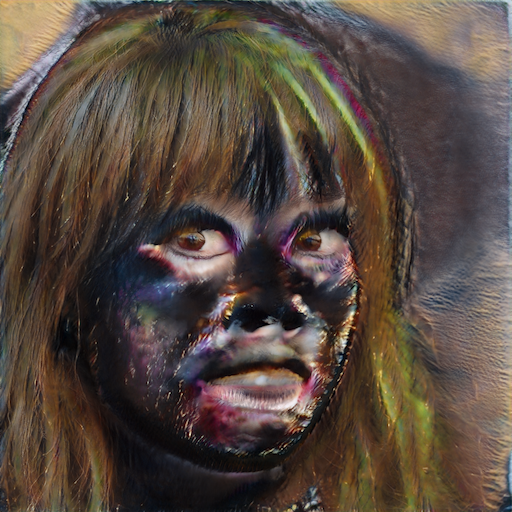
\includegraphics[width=.24\textwidth]{figures/c5_netbend/cluster_comparison/layer_10_cluster0_mult-1.png}}
        \hfill
        \subfloat[]{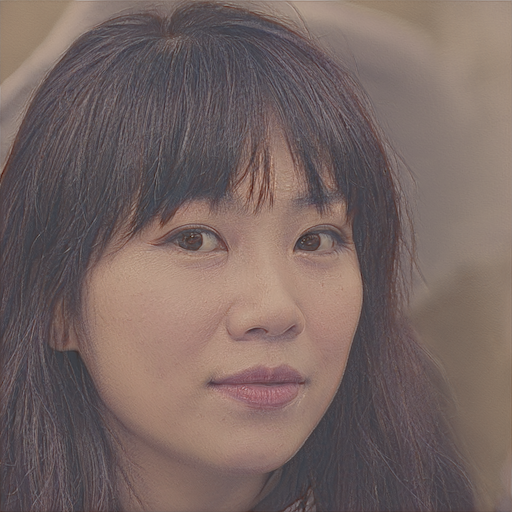
\includegraphics[width=.24\textwidth]{figures/c5_netbend/cluster_comparison/layer_15_cluster0_mult0.1.png}}
       \caption[A comparison of different transforms being applied to different clusters in various layers of StyleGAN2]{Examples from the clustering algorithm in the image domain. Clusters of features in different layers of the model are responsible for the formation of different image attributes. (a) The unmanipulated result. (b) A cluster in layer 1 has been multiplied by a factor of -1 to completely remove the facial features. (c) A cluster in layer 3 has been multiplied by a factor of 5 to deform the spatial formation of the face. (d) A cluster in layer 6 has been ablated to remove the eyes. (e) A cluster in layer 6 has been dilated with a structuring element with radius $r=2$ pixels to enlarge the nose. (f) A cluster in layer 9 has been multiplied by a factor of 5 to distort the formation of textures and edges. (g) A cluster of features in layer 10 has been multiplied by a factor of -1 to invert the highlights on facial regions. (h) A cluster of features in layer 15 has been multiplied by a factor of 0.1 to desaturate the image. All transformations have been applied to sets of features discovered using the feature clustering algorithm (\S\ref{c5:section:clustering}) in the StyleGAN2 model trained on the FFHQ dataset.}
       \label{fig:c5:cluster_layer_comp_image}
    \end{figure}

The main motivation of the clustering algorithm presented in this paper was to simplify the parameter space in a way that allows for more meaningful and controllable manipulations whilst also enhancing the expressive possibilities afforded by interacting with the system. 
These results show that the clustering algorithm is capable of discovering groups of features that correspond to the generation of different semantic aspects of the results, which can then be manipulated in tandem. 
These semantic properties are discovered in an unsupervised fashion and across the entire hierarchy of features present in the generative model.
Figure \ref{fig:c5:cluster_layer_comp_image} shows the manipulation of groups of features across a broad range of layers that control the generation of the entire face, the spatial formation of facial features, the eyes, the nose, textures, facial highlights and overall image contrast.

\section{Manipulation Pipeline}

Transforms are specified in YAML (YAML Ain't Markup Language) configuration files \citep{ben2009yaml} (Fig. \ref{fig:c5:yaml-transform-config} for an example of one of these configs), such that each transform is specified with 5 items: (i) the layer, (ii) the transform itself, (iii) the transform parameters, (iv) the layer type (i.e. how the features are selected in the layer: across all features in a layer, to pre-defined clusters, or to a random selection of features), and (v) the parameter associated with the layer type (either the cluster index, or the percentage of features the filter will randomly be applied to). 
Visual examples of how different layer types can be seen in Figure \ref{fig:c5:layer-transform-types}.
There can be any number of transforms defined in such a configuration file and transforms can be chained together to produce more complex filtering effects in the generated output  (Fig. \ref{subfig:chaining-transformations}).

After loading the configuration, the software either looks up which features are in the cluster index or randomly applies indices based on the random threshold parameter. 
Then the latent is loaded, which can either be randomly generated, or be predefined in latent space $z$, or be calculated using a projection in latent space $w$ \citep{abdal2019image2stylegan,karras2019analyzing} (in the case of StyleGAN2). The latent code is provided to the generator network and inference is performed. 
As this implementation is using PyTorch \citep{paszke2019pytorch}, a dynamic neural network library, these transformation layers can therefore be inserted dynamically during inference as and when they are required and applied only to the specified features as defined by the configuration. 
Once inference is unrolled, the generated output is returned. Figure \ref{fig:c5:overview_diagram} provides a visual overview of the pipeline, as well as a comparison between a modified and unmodified generated sample.

\begin{figure}[!htb]
    \centering
    \subfloat[]{\label{subfig:layer-wide}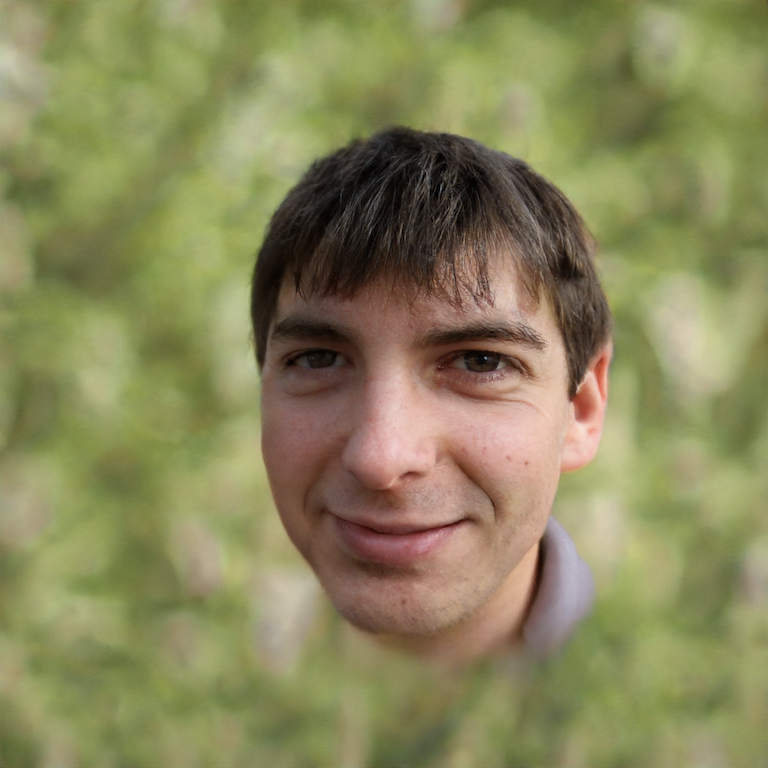
\includegraphics[width=.24\textwidth]{figures/c5_netbend/layer-transform-types/layer-wide.png}}
    \hfill
    \subfloat[]{\label{subfig:random-layer}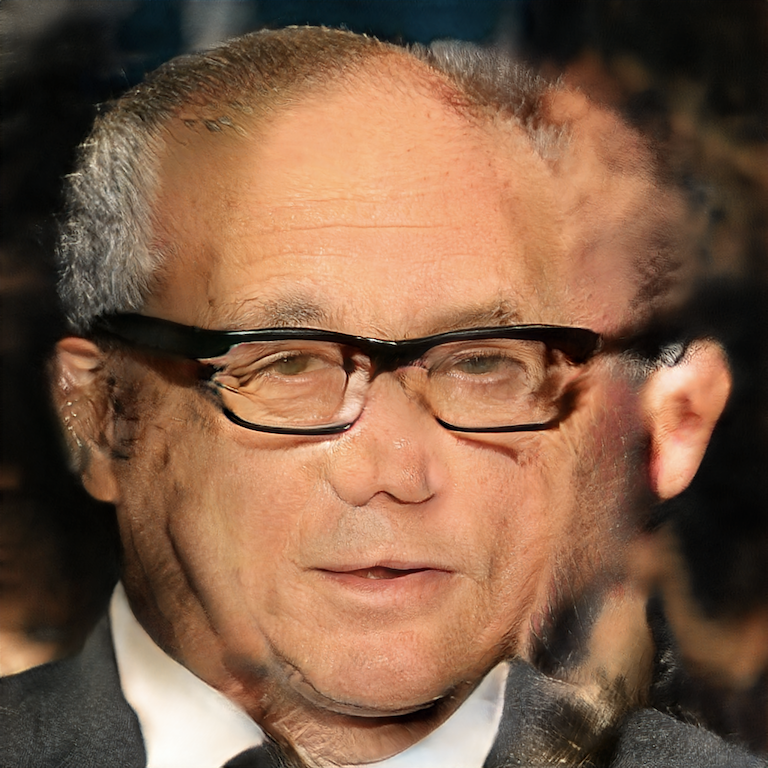
\includegraphics[width=.24\textwidth]{figures/c5_netbend/layer-transform-types/stochastic.png}}
    \hfill
    \subfloat[]{\label{subfig:cluster-layer}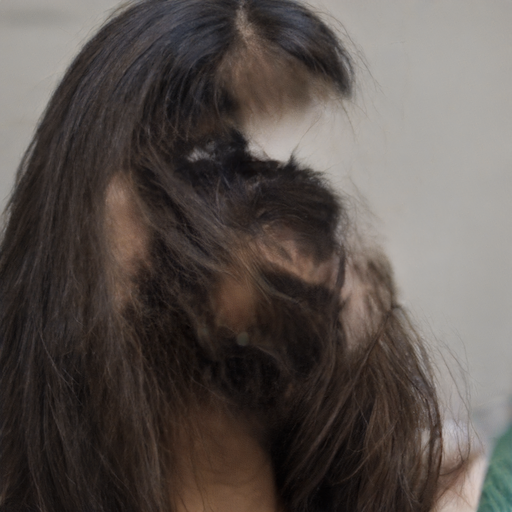
\includegraphics[width=.24\textwidth]{figures/c5_netbend/layer-transform-types/cluster.png}}
    \hfill
    \subfloat[]{\label{subfig:chaining-transformations}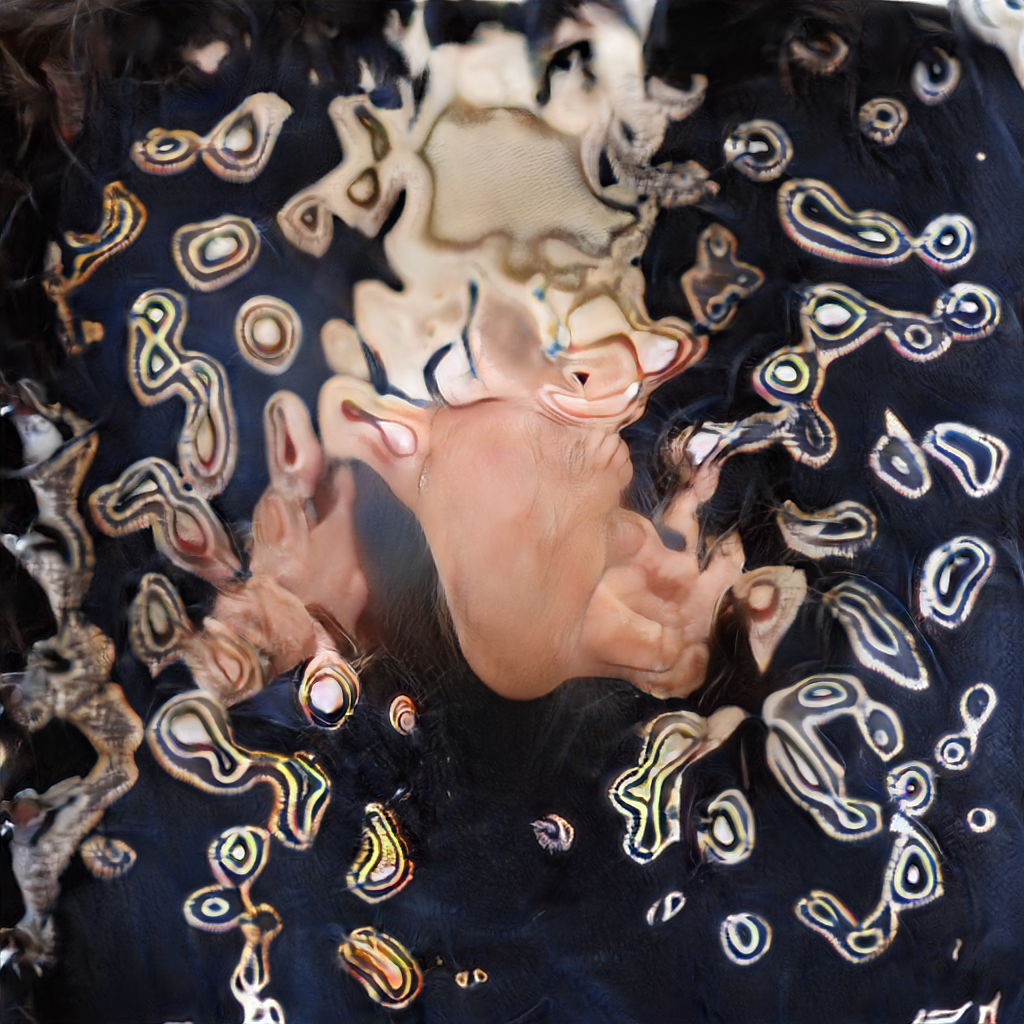
\includegraphics[width=.24\textwidth]{figures/c5_netbend/layer-transform-types/chaining-transforms.png}}
    \caption[Examples of transformation layers being applied to different configurations of features]{Examples of transformation layers being applied to different configurations of features in StyleGAN2. (a) Transformation applied layer-wide. (b) Transformation is applied to a random selection of filters in one layer. (c) Transformation applied to a cluster in layer 2. (d) A combination of transformation layers applied across a network, the configuration of transformations used to generate this image can be seen in Figure \ref{fig:c5:yaml-transform-config}.}
    \label{fig:c5:layer-transform-types}
 \end{figure}

 \begin{figure}[!htb]
 \begin{lstlisting}[language=yaml]
    ---
    transforms:
    - layer: 2
      transform: "invert"
      params: []
      features: "all"
      feature-param: 
    - layer: 6
      transform: "binary-thresh"
      params: [0.5]
      features: "random"
      feature-param: 0.5
    - layer: 6
      transform: "scalar-multiply"
      params: [5]
      features: "cluster"
      feature-param: 2
    ---
    \end{lstlisting}
    \caption[Example YAML transformation config]{Example of a YAML transformation config that is used in the network bending framework. This config combines randomly applied layers and layer-wide transformations. This config was used to generate the image Figure \ref{subfig:chaining-transformations}.}
    \label{fig:c5:yaml-transform-config}
 \end{figure}

\section{Network Bending in the Audio Domain}
\label{c5:sec:net-bend-audio}

As a follow-up study to the original network bending approach on images, I applied the same approach to the audio domain as an extension to the work for the journal paper in Entropy \citep{broad2022network}. 
The motivation for this was to demonstrate that network bending was applicable to different types of media and to demonstrate the general-purpose nature of this framework. 

For this study, I trained a custom VAE model on spectrograms of music and applied the exact same algorithm for clustering and applying the same transformation layers as was applied in network bending for image generation. 
Network bending has also been applied to audio by other researchers and practitioners, this efforts are detailed in Sections \ref{c7:subsubsec:naotokui} \& \ref{c7:subsubsec:ddsp}.

\subsection{Custom Audio Model}

For this experiment, I trained a variational autoencoder (VAE) \citep{kingma2013auto,rezende2014stochastic} on spectrograms extracted from a custom dataset of varied musical genres, totalling 3461 audio tracks. This approach is based on previous methods for learning generative models of spectrograms \citep{akten2018granma} and Mel spectrograms \citep{valenzuela2021melspecvae} with VAEs. The tracks are randomly split up into short sequences and the Fourier transform is performed with a hop size of 256 and a window size of 1024 to produce spectrograms that have a bin size of 513. The spectrograms are then cut into shorter sequences of a window length of 128. These shortened spectrograms are then converted to decibels and then normalised for training with the VAE.  

The VAE was built using a convolutional architecture with a latent vector with dimension $\vec{v} \in \mathbb{R}^{512}$. The encoder has 5 layers that use standard convolutions with a kernel size of 5x5, a stride of 2x2 and no padding for all of the layers. The decoder uses transposed convolutions, and table \ref{tab:c5:decoder-architecture} lists the output resolution, kernel size, stride, and padding parameters for each of the 5 convolutional layers. A fully connected layer is used in both the encoder and decoder to interface between the convolutional layers and the latent vector. The model was trained for 50 epochs on the dataset with batch normalisation using a batch size of 64. The model was trained using the Adam optimiser \citep{kingma2014adam} with a learning rate of 0.0003 and with $\beta_1 = 0$ and $\beta_2 = 0.99$.

After training it is possible to sample randomly in the latent space and then sample directly from the decoder. It is also possible to input audio sequences, both from the training set and outside of it, and produce reconstructions of the audio track mediated through the VAE model, in a method that I have previously referred to as \textit{autoencoding} \citep{broad2017autoencoding}. Performing this autoencoding procedure in combination with network bending, provides a new way of transforming and filtering audio.

\begin{table*}[]
    \centering
    \begin{tabular}{|c|c|c|c|c|c|c|c|}
    \hline
    Layer & Resolution & \#features & kernel size & stride & padding \\
    \hline
    1     & 8x33       & 512        & 5x5         & 1x2     & 0x2  \\
    2     & 17x65      & 256        & 3x5         & 2x2     & 2x2 \\
    3     & 32x129     & 128        & 4x5         & 2x2     & 2x2 \\
    4     & 64x257     & 64         & 4x5         & 2x2     & 2x2  \\
    5     & 128x513    & 1          & 4x5         & 2x2     & 2x2  \\
    \hline
    \end{tabular}
    \medskip
    \caption{\label{tab:c5:decoder-architecture}Table showing resolution, number of features of each layer, convolutional kernel size, strides, and padding parameters for the decoder network in the spectrogram VAE.}
    
    \end{table*}

\subsection{Clustering}

the approach to clustering for this audio model was identical to what was demonstrated in Section \ref{c5:section:clustering}.
As the VAE model did not have as many layers as StyleGAN2, clusters were only calculated for four layers, the details of which can be seen in Table \ref{tab:c5:audio-clustering}.

\begin{table*}[]
    \centering
    \begin{tabular}{|c|c|c|c|c|c|c|c|}
    \hline
    Layer & CNN Depth & \#clusters \\
    \hline
    1     & 1 &   5 \\
    2     & 2 &   5 \\
    3     & 3 &   4 \\
    4     & 4 &  4 \\
    \hline
    \end{tabular}
    \medskip
    \caption{\label{tab:c5:audio-clustering}Table showing the number of ShuffleNet \citep{zhang2018shufflenet} convolutional blocks for each CNN model used for metric learning and the number of clusters calculated for each layer using $k$-means.}
    
    \end{table*}

\subsection{Results}

The clustering approach applied to the audio model appears to work well when visualising the spectrograms, and it is clear that this approach can capture and manipulate some semantically meaningful components in the audio signal\footnote{Unfortunately there was a bug in the decoding of the spectrograms back into audio which meant that the audio quality in the generated samples was very noisy -- something that I have not been able to fix.}  (Fig. \ref{fig:c5:cluster_audio_comp}). 
Not all of the transformations that can be applied to images work as well in audio, such as scaling and rotation.
This is not a surprise given that the location of each pixel is essential information used to represent frequency and time information in the audio signal, and can completely transform the information represented when manipulated.
However, the morphological transformations do at least preserve locality in the signal, and using these filters in generative models of spectrograms offers a completely new way to transform audio signals.

\begin{figure}[tp!]
\vspace{-80pt}
\centering
    \subfloat[]{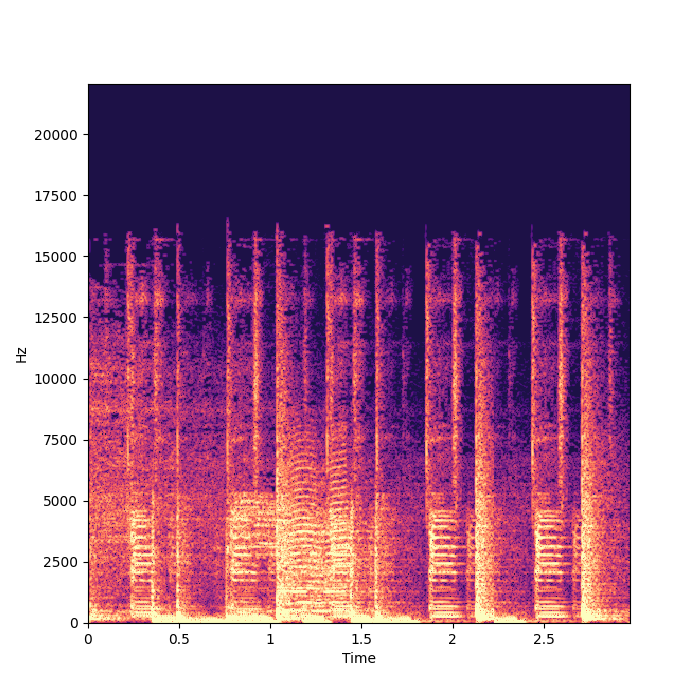
\includegraphics[width=.4\textwidth]{figures/c5_netbend/audio_clusters/soul_short_original.png}}
    \hfill
    \subfloat[]{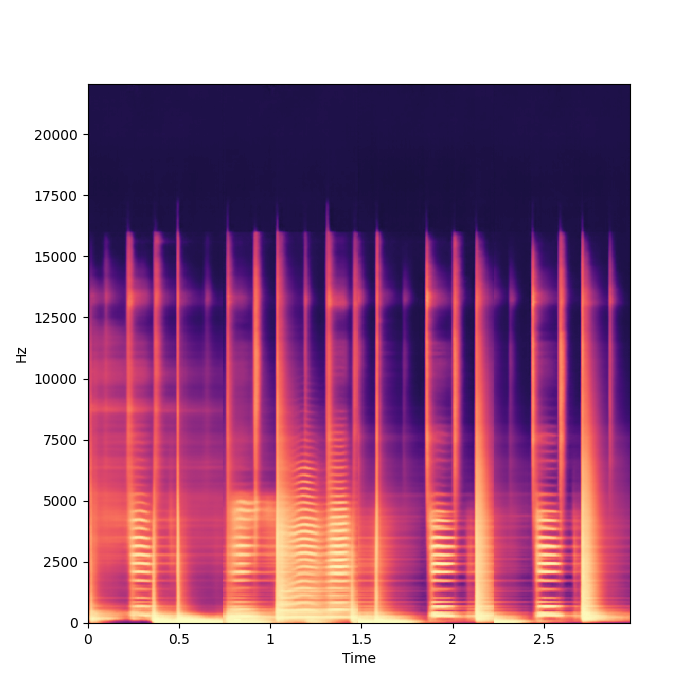
\includegraphics[width=.4\textwidth]{figures/c5_netbend/audio_clusters/soul_short_reconstruction.png}}
   \hfill
    \subfloat[]{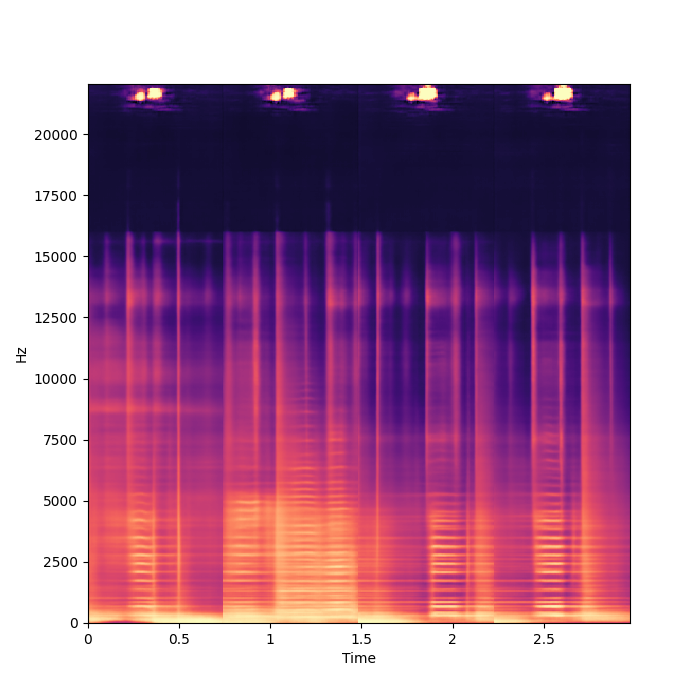
\includegraphics[width=.4\textwidth]{figures/c5_netbend/audio_clusters/layer_1_cluster3_ablate.png}}
    \hfill
    \subfloat[]{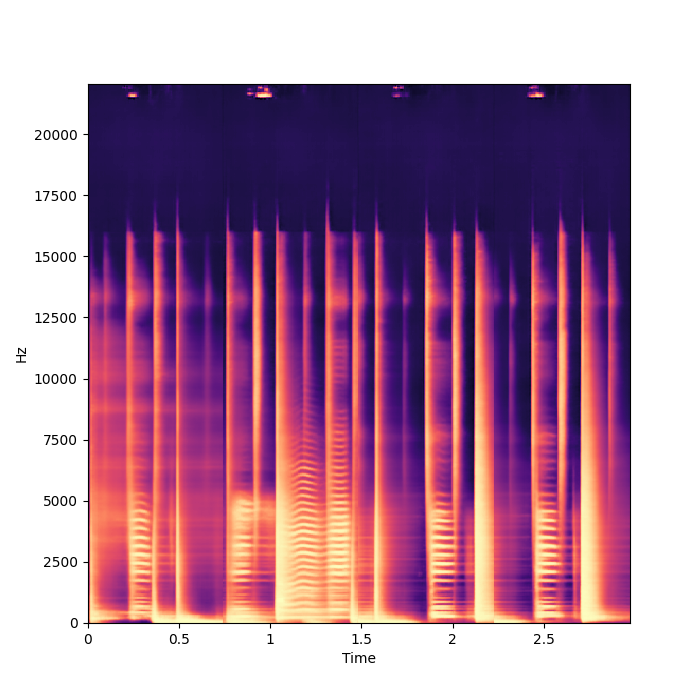
\includegraphics[width=.4\textwidth]{figures/c5_netbend/audio_clusters/layer_1_cluster3_mult_2.png}}
   \hfill
    \subfloat[]{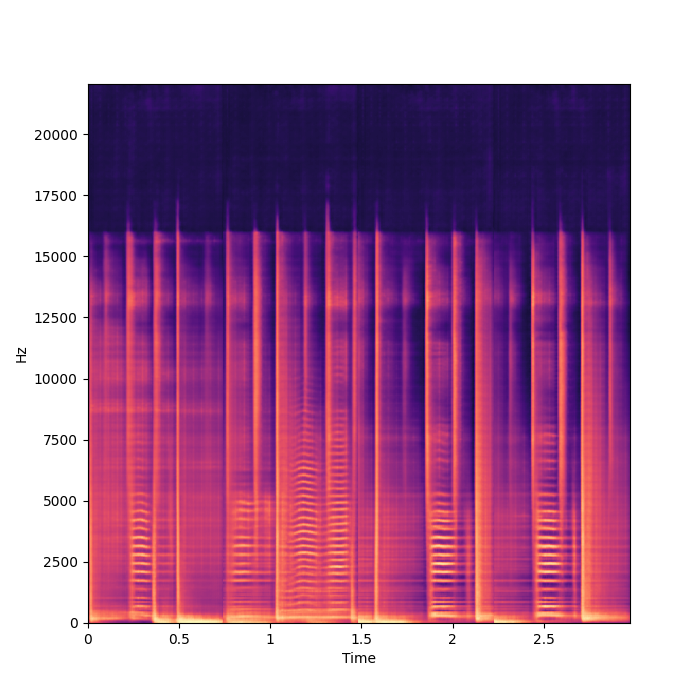
\includegraphics[width=.4\textwidth]{figures/c5_netbend/audio_clusters/layer_3_cluster2_erode.png}}
    \hfill
    \subfloat[]{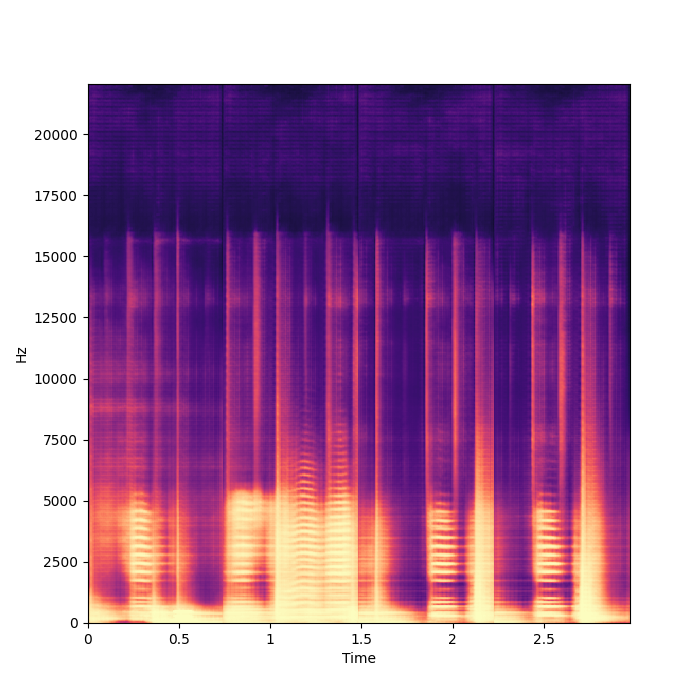
\includegraphics[width=.4\textwidth]{figures/c5_netbend/audio_clusters/layer_3_cluster2_dilate.png}}
   \caption[A comparison of different transforms being applied to different clusters in various layers of the SpectrogramVAE]{Examples from the clustering approach in the audio domain. (a) Spectrogram of an original source track not in the training set. (b) Reconstruction of source track using VAE without manipulation. (c) Reconstruction of the same signal where a cluster in layer 1 responsible for the generation of the transients of the signal has been ablated. (d) Reconstruction of the same signal where the same cluster in layer 1 responsible for the transients has been multiplied by a factor of 2, increasing the intensity of the transients in the resulting signal. (e) Reconstruction of the signal where a cluster in layer 3 responsible for the low and mid-range frequencies has been eroded with a structuring element with radius $r=2$ pixels, diminishing the intensity of these frequency components. (f) Reconstruction of the signal where the same cluster in layer 3 responsible for the low and mid-range frequencies has been dilated with a structuring element with radius $r=2$ pixels, increasing the intensity of these frequency components. The audio sample used is a clip from \textit{Saulsalita Soul} by Mr.RuiZ, reproduced and transformed with permission granted under the CC BY-NC 4.0 licence.}
   \label{fig:c5:cluster_audio_comp}
\end{figure}

\section{Discussion}

In this section, I discuss several different perspectives on the outcomes presented here: expressive manipulation, active divergence, comparisons of the results between the image and audio domains, and comparisons with other methods.

\subsection{Expressive Manipulation}

The main motivation of the clustering algorithm presented in this chapter was to simplify the parameter space in a way that allows for more meaningful and controllable manipulations whilst also enhancing the expressive possibilities afforded by interacting with the system. 
These results show that the clustering algorithm is capable of discovering groups of features that correspond to the generation of different semantic aspects of the results, which can then be manipulated in tandem. 
These semantic properties are discovered in an unsupervised fashion and across the entire hierarchy of features present in the generative model.
For example, Figure \ref{fig:c5:cluster_layer_comp_image} shows the manipulation of groups of features across a broad range of layers that control the generation of the entire face, the spatial formation of facial features, the eyes, the nose, textures, facial highlights and overall image contrast. Figure \ref{fig:c5:cluster_audio_comp} shows the clustering algorithm performed in the audio domain, to demonstrate how aspects of the audio signal such as the transients and frequency components can be manipulated with various kinds of transformations.

Grouping and manipulating features in a semantically meaningful fashion is an important component of allowing expressive manipulation. 
However, artists are often also ready to consider surprising, unexpected results, to allow for the creation of new aesthetic styles, which can become uniquely associated with an individual or group of creators. 
Therefore the tool needs to allow for unpredictable as well as predictable possibilities, which can be used in an exploratory fashion and can be mastered through dedicated and prolonged use \citep{dobrian2006nime}. 
There is usually a balance between the utility and expressiveness of a system \citep{jacobs2017supporting}. 

Section \ref{c7:sec:net-bend-artworks} shows the various different ways this framework has been used to make artworks.
Whilst I did not make a user interface for network bending myself, many other researchers have gone on to do so.
Their efforts are detailed in \S \ref{c7:subsec:net-bend-interfaces}.

\subsection{Comparison Between Audio and Image Domains}

In this chapter, I have described the network bending framework in both the image and audio domains. 
For the image domain, I have used StyleGAN2 \citep{karras2019analyzing}, the state of the art generative model for unconditional image generation. In the audio domain, I have built a custom generative model to demonstrate how the same principles of clustering features and applying transformations to clustered features can be applied indirectly to another domain. 
The generative model for audio I have presented is building on a much smaller body of research and has more room for improvement in terms of the fidelity of the generated outputs, however, it is still adequate and demonstrates that the clustering algorithm is capable of discovering semantically meaningful components of the signal  (Fig. \ref{fig:c5:cluster_audio_comp}). 
Some of the transformation layers that were designed for image-based models such as rotation and scaling do not transfer meaningfully into the audio domain. 
However, numerical and morphological transformations do work effectively in the audio domain, representing a completely new approach for manipulating audio signals. 
In addition to my efforts, other researchers have also gone on to successfully implement network bending in audio models (\S \ref{c7:subsubsec:naotokui} \& \S \ref{c7:subsubsec:ddsp}).

\subsection{Comparison with Other Methods}

With respect to the semantic analysis and manipulation of a generative model, this approach of clustering features and using a broad array of transformation layers is a significant advance over previous works \citep{Bau2017-vg,Bau2018-td,bau2019semantic, Brink2019-gc}. 
This recent thread of techniques only interrogates the function of individual features, and as such is unlikely to be capable of capturing a full account of how a deep network generates results since such networks tend to be robust to the transformation of individual features. 

The results in this chapter show that sets of features, which may not be particularly responsive to certain transformations, are very responsive to others. 
Figure \ref{fig:c5:ablation_comp} shows that in the model trained on the LSUN church dataset, a cluster of features, when ablated, have little noticeable effect on the result.
However, significant changes are visible when using the pointwise scalar multiplication transformation on the same cluster, here removing the trees and revealing the church building that was obscured by the foliage in the original result. 
The clustering approach described in this paper suggests that the functionality of features, or sets of features, cannot be understood only through ablation, because of the high levels of redundancy present in the learned network parameters. 
In addition, the research here shows that their functionality can be better understood by applying a wide range of deterministic transformations, of which different transformations, some of which are better suited to revealing the utility of different sets of features (Figs. \ref{fig:c5:cluster_layer_comp_image} \& \ref{fig:c5:ablation_comp}). 
An approach that has since been developed further by \cite{oldfield2022panda,oldfield2024bilinear}.

\begin{figure}[!htbp]
   \centering
   \subfloat[]{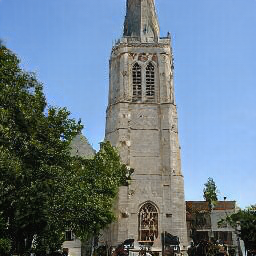
\includegraphics[width=.32\textwidth]{figures/c5_netbend/church_ablation_comparison/not_manipulated.png}}
   \hfill
   \subfloat[]{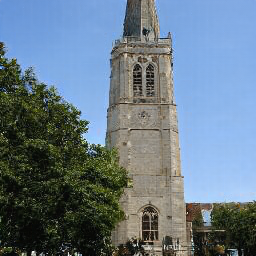
\includegraphics[width=.32\textwidth]{figures/c5_netbend/church_ablation_comparison/layer_3_cluster1_ablate.png}}
   \hfill
   \subfloat[]{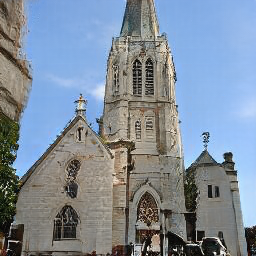
\includegraphics[width=.32\textwidth]{figures/c5_netbend/church_ablation_comparison/layer_3_cluster1_mult5.png}}
   \caption[A comparison of one cluster in StyleGAN2 having two different transforms applied to it]{Groups of features that are not particularly sensitive to ablation may be more sensitive to other kinds of transformation. (a) Original unmodified input. (b) A cluster of features in layer 3 that has been ablated. (c) The same cluster of features that has been multiplied by a scalar of 5. As can be seen, ablation had a negligible effect, only removing a small roof structure that was behind the foliage. On the other hand, multiplying by a factor of 5 removes the trees whilst altering the building structure to have gable roof sections on both the left and right sides of the church - which are now more prominent and take precedence in the generative process. Samples are taken from the StyleGAN2 model trained on the LSUN church dataset.}
   \label{fig:c5:ablation_comp}
\end{figure}

This method of analysis is completely \emph{unsupervised} and does not rely on auxiliary models trained on large labelled datasets (such as in \citep{Bau2018-td, isola2017image, park2019semantic}) or other kinds of domain-specific knowledge. 
This approach therefore can be applied to any CNN-based generative model architecture which has been trained on any dataset, as I have demonstrated by using the exact same clustering method for both image and audio domains. 
This is of particular relevance to artists who create their own datasets and would want to apply these techniques to models they have trained on their own data. 
Labelled datasets are prohibitively time-consuming (and expensive) to produce for all but a few individuals or organisations. 
Having a method of analysis that is completely unsupervised and can be applied to unconditional generative models is important in opening up the possibility for such techniques to become adopted more broadly.
Section \ref{c7:sec:net-bend-artworks} details a number of artworks made by myself and others, applied to a range of datasets, both preexisting and custom.
The limitation of this approach is the time and computational resources needed to train a separate model for each layer of the network.
This limitation is discussed further in Section \ref{c9:sec:limitations}, and ways to improve upon this are further presented in Section \ref{c9:sec:future}.


\section{Conclusion}

In this chapter, I have introduced a novel approach for the interaction with and manipulation of generative neural networks, which has been demonstrated in both the image and audio domains. 
By inserting deterministic filters inside pre-trained neural networks, this framework allows for manipulation to be performed inside the networks' `black-box', generating samples that have no resemblance to the training data, or anything that could be created easily using conventional media editing software. 
This chapter also presents a novel clustering algorithm that can group sets of features in an unsupervised fashion, based on the spatial similarity of their activation maps. 
I have demonstrated that this method is capable of finding sets of features that correspond to the generation of a broad array of semantically significant aspects of the generated results in both image and audio domains. 

The goal of the work in this thesis was to find a way to expand the possibility space of what can be generated with neural networks.
\textit{Network bending} is an approach that expands the generative space of existing pre-trained models in a way that gives direct control and agency to artists and creative practitioners, and in a way that \textit{actively diverges} from data.
This now concludes the documentation of new algorithms and approaches to \textit{active divergence} presented in this thesis. 
The next chapter will a broader perspective, contextualising the work in this thesis with other related efforts that occurred during its development.
Chapter \ref{ch:active_div} gives a detailed survey and taxonomy of active divergence methods, placing the work presented in this thesis into a larger context and delineating and outlining the landscape of active divergence methods to date. 
